\section{Megvalósítások}
Első részben a megvalósításokat natív HTML CSS és JavaScript elemekkel próbáltam megoldani. Ez volt az az időszak amikor elkezdtem utána nézni, hogy a céljaim közül mi valósítható meg és mi nem. Az első amivel bővebben kezdtem foglalkozni maga a 3D modell betöltése volt egy web oldalra. Idő közben rájöttem, hogy natív HTML-be nem tudok beimportálni egy 3D objektumot. Kerestem keretrendszereket ahol tudok használni ilyen jellegű modelleket. Először Angular keretrendszerben próbáltam ki. Itt elég sok időt eltöltöttem, hogy megtudjam jeleníteni az objektumot de sikerült.

Tovább kutatva megtaláltam a Vue.js keretrendszert is. Ebben már egyszerűbb volt a 3D objektum beillesztése mivel az Angularhoz hasonlónak kellet volna lennie. Viszont Vue.js-ben találtam kimondottan egy csomagot(package) amely direkt ilyen jellegű modellekkel foglalkozott. Ezek után a 3D modell megjelenítése már hamar megtörtént. 

Ezt követően neki fogtam tanulmányozni, hogy mit is tudok kezdeni egy ilyen modellel. Első körben megtanultam betölteni a weboldalra. Majd tovább keresve már tudtam forgatni is az elemet. A közelítés és a távolítás alapból beépítve található a csomagban így ennek nem kellett utána keresnem.

A projektem egyik legfontosabb része, hogy egy 3D modellt tudjak beépíteni, kezelni lassan kezdett megvalósulni így elkezdtem készíteni egy demo-t ahol az elképzeléseimet próbáltam összeszedni, megjeleníteni. Ez egy hosszabb folyamatnak bizonyult viszont a végére kezdett körvonalazódni, hogy fog kinézni maga az alkalmazás. A demo elkészítését már csak Vue.js keretrendszeren belül készítettem el.

Mindezek után ráébredtem, hogy lassan neki kellene fognom az eredeti projektnek is. Így neki kezdtem lefejleszteni a demoban elképzelt ötleteimet. Először a visitor(látogató) felhasználók oldalát kezdtem elkészíteni. Itt rájöttem, hogy kellene nekem egy adatbázis és a backend rész is amely segítségével tudok az adatbázisban szereplő adatokkal dolgozni. Úgy döntöttem, hogy a frontend és backend részt párhuzamosan fogom elkészíteni.

Annak érdekében, hogy a frontend és backend részt tudjam párhuzamosan fejleszteni szükségem volt egy adatbázisra. Így neki fogtam elkészíteni az adatbázisomat. Először megterveztem a tábláimat majd megpróbáltam minden hibát kiküszöbölni. Úgy gondolom, hogy ezek a táblák még nem tökéletesek, lesz még változtatás rajtuk de egyelőre az elinduláshoz szükségesek. Az \ref{fig:database} ábrán láthatóak az adatbázis táblák. Láthatjuk, hogy kilenc tábla hozódott létre különböző kapcsolatokkal. Az admin tábla tartalmazza azokat a felhasználókat, amelyek be tudnak jelentkezni. A branch tábla tartlamzza a részlegket mint például a tanszékek, vagy a dékáni hivatal. Itt összeköttetés figyelhetünk meg két táblával is. A contactperson tábla megadja a kapcslattartó személyt míg a department tábla meghatározza a alrészlegeket mint például a szakok. Tovább tekintve láthatunk egy file nevű táblát ami fájlokat. Észrevehető, hogy ez a tábla is kapcsolatot teremt három különböző táblával. Az első tábla neve event amely már el is árulja hogy az eseményekhez kapcsolodó adatokat, információkat tartalmazza. A második tábla a headerimg amely a fejlécen megjelenő képet tárolja. Harmadik tábla a model amely maga a 3D modell-t leíró adatokat tárolja.
\begin{figure}
	\centering
	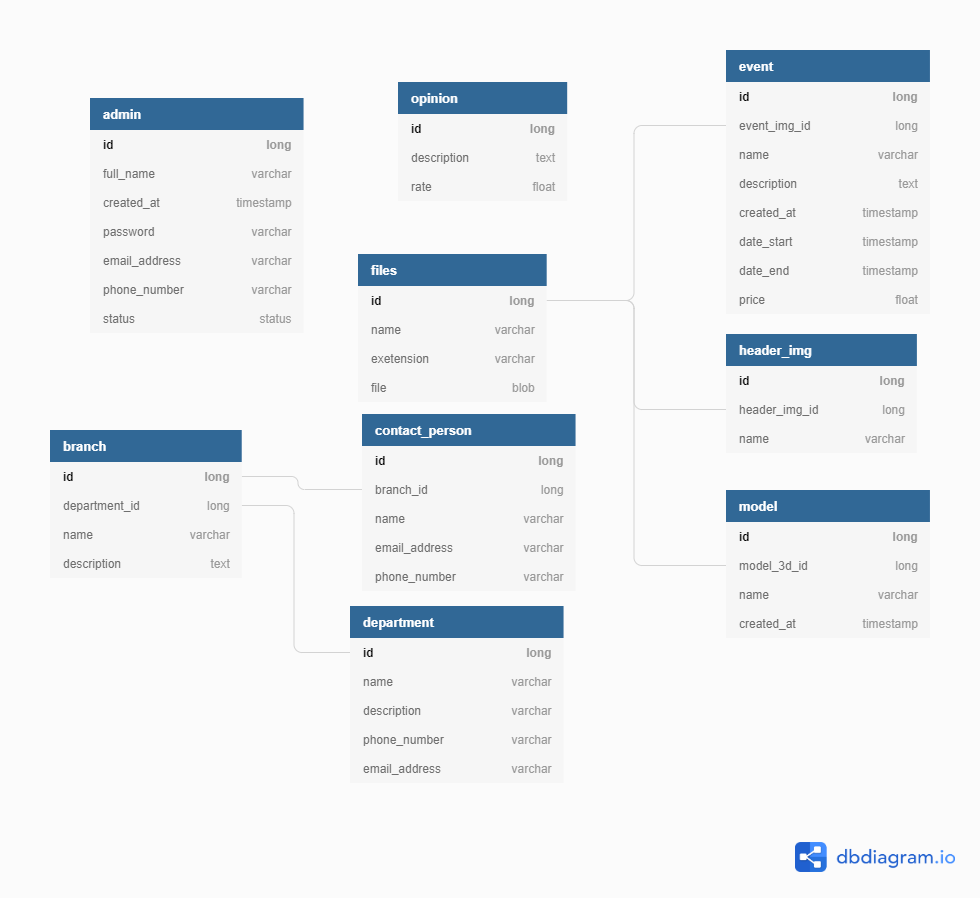
\includegraphics[scale=0.3]{figures/images/Sapi3dTour.png}
	\caption{Az adatbázist alkotó táblák.}
	\label{fig:database}
\end{figure}

Az adatbázis megtervezés után, neki fogtam a backend részt elkezdeni. Ehhez Spring Bootot használtam ami megkönnyíti az adatbázis létrehozásának folyamatát. A kódot Java-ban kell írni és minden tábla egy osztálynak felel meg. A Spring Boot tanulmányozása során jöttem rá, hogy mennyire oda kell figyelni a különböző annotációkra. Kis idő elteltével elsajátítottam a Spring Boot struktúráját és ezt használva felépítettem a backend rész első fázisát. Az adatbázis egyelőr PostgreSQL-ben van létrehozva viszont a Spring segítségével gyorsan bármely adatbázissal lehet kapcsolatot teremteni.

Mindeközben fejlesztettem a frontend részt is. Eljött az a pillanat, hogy kapcsolatot kellett teremtenem a frontend és a backend rész között, amelyet hamar sikerült elvégeznem. Így már tudott kommunikálni a frontend a backenddel vagyis a frontendre az adatbázisban szereplő adatok eljutottak és jelentek meg a weboldalon. 

A következő részben látható lesz képek formájában a forntend rész haladata. Az első részben bemutatnám, hogy a user felhasználók mit látnak. Első sorban a menürendszerrel kezdeném. Ha már be van jelentkezve egy felhasználó akkor a \ref{fig:drawbar} ábrán látható menü rendszerrel fog találkozni. Megfigyelhető, hogy megjelennek a felhasználó adatai és egy gomb amely segítségével tudja módosítani az adatait.Erről képet láthatunk a \ref{fig:changedata} ábrán. Ezek után jönnek a lehetőségek amelyekre rákattintva különböző oldalak jelennek meg.
\begin{figure}
	\centering
	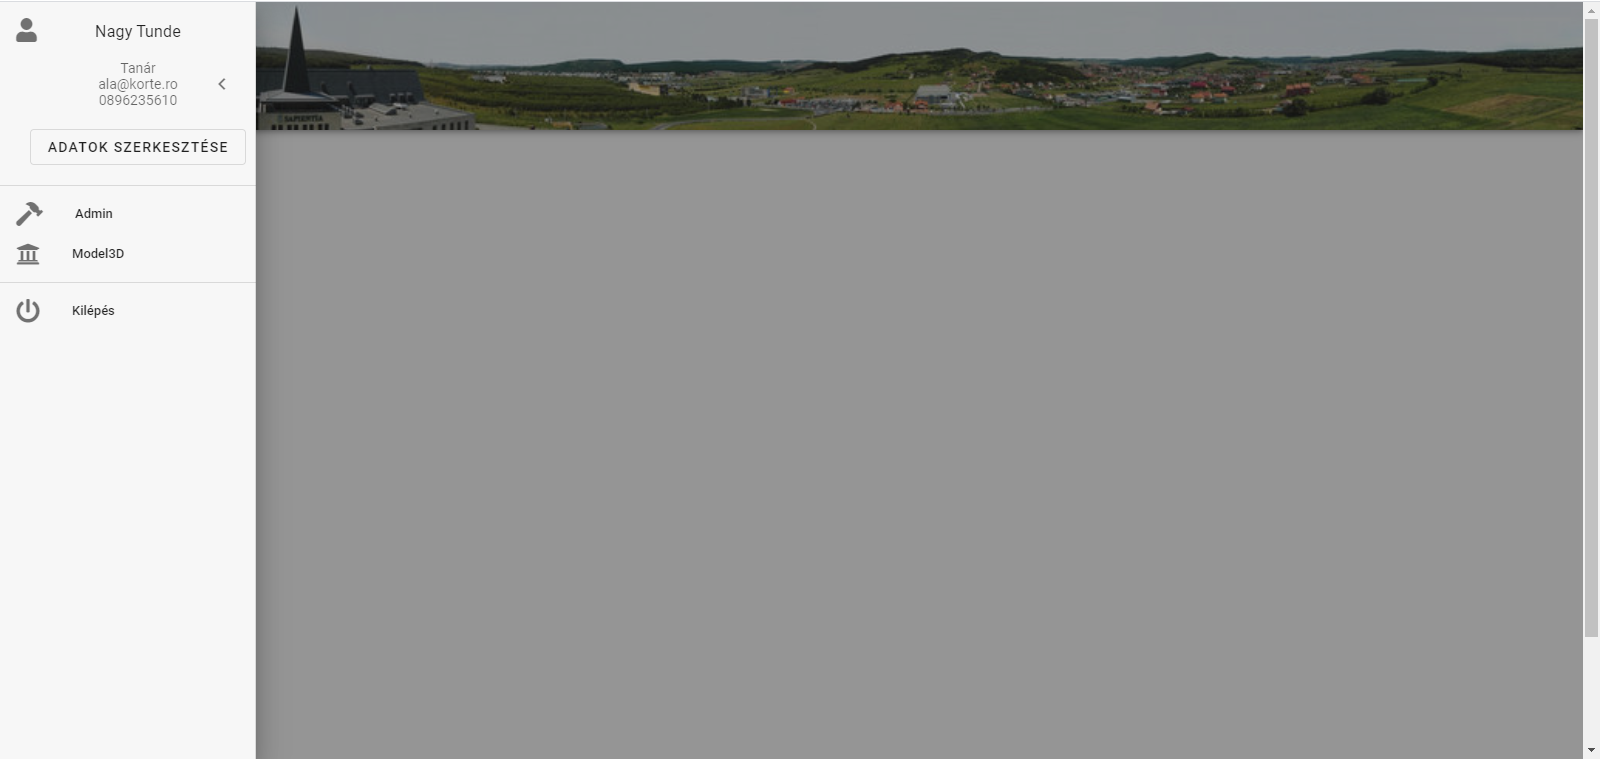
\includegraphics[scale=0.4]{figures/images/drawbar.png}
	\caption{A user felhasználók menü rendszere}
	\label{fig:drawbar}
\end{figure}
\begin{figure}
	\centering
	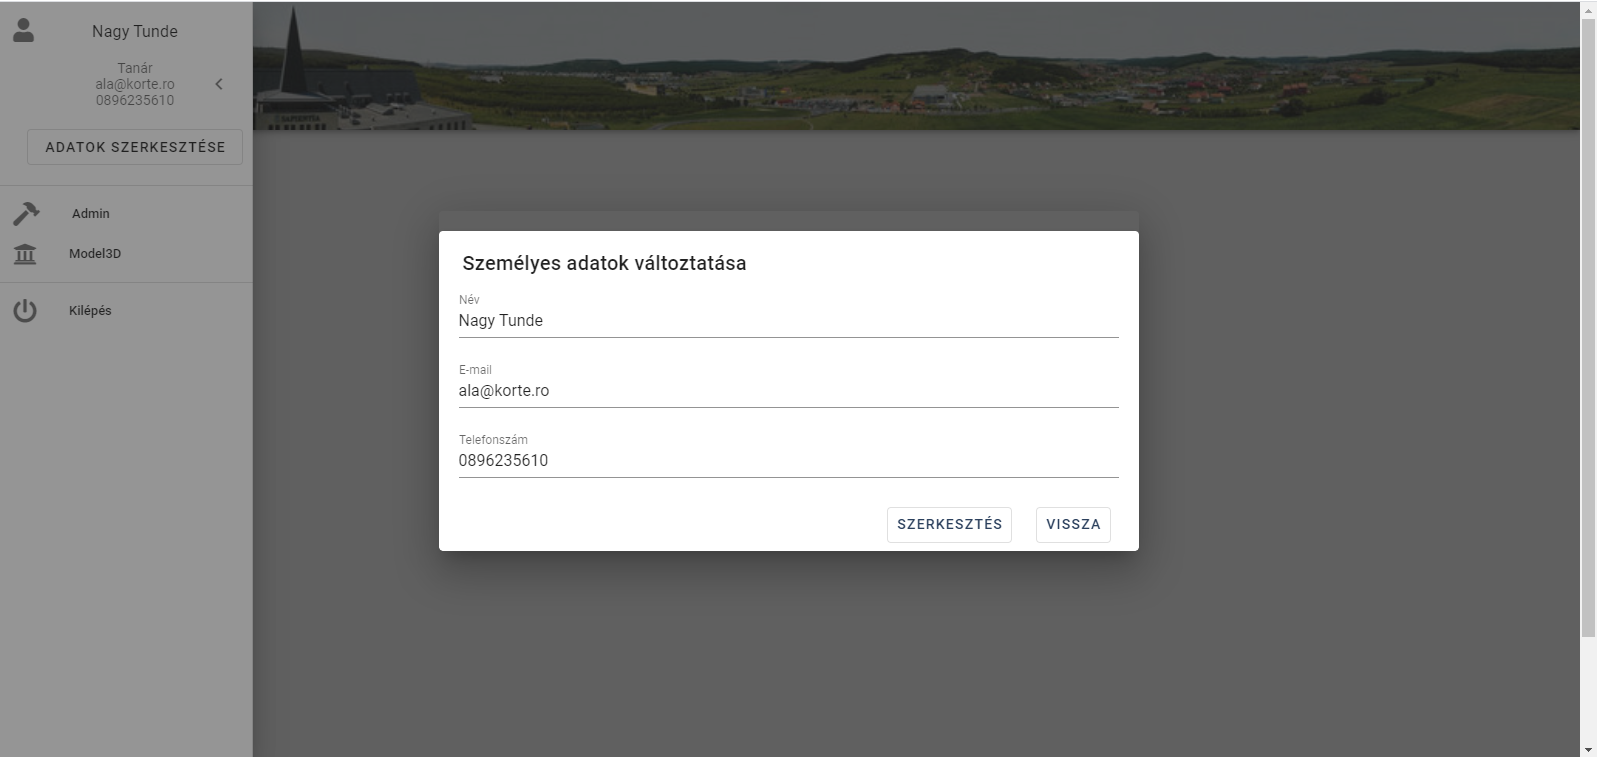
\includegraphics[scale=0.4]{figures/images/changedata.png}
	\caption{A user felhasználók adatainak módosítása}
	\label{fig:changedata}
\end{figure}
	
A menürendszer első opcióját választva vagyis az Admin opciót akkor előjönnek azok a funkcionalitások, amelyeket eltud végezni a felhasználó annak függvényében hogy milyen joggal rendelkezik. Egyelőre csak az új user felhasználók hozzáadása működik, amelyhez csak annyit kell tennünk, hogy beírjuk az adatokat és ráklikkelünk a HOZZÁADÁS gombra. Ez által bekerül az új felhasználó az adatbázisba. Erről az oldalról a \ref{fig:admin} ábrán láthatunk egy képet. Az utolsó menü pont a kijelentkezés gomb amely segítségével a felhasználó ki  tud jelentkezni és vissza kerül arra az oldalra amelyet már minden felhasználó képes látni.
\begin{figure}
	\centering
	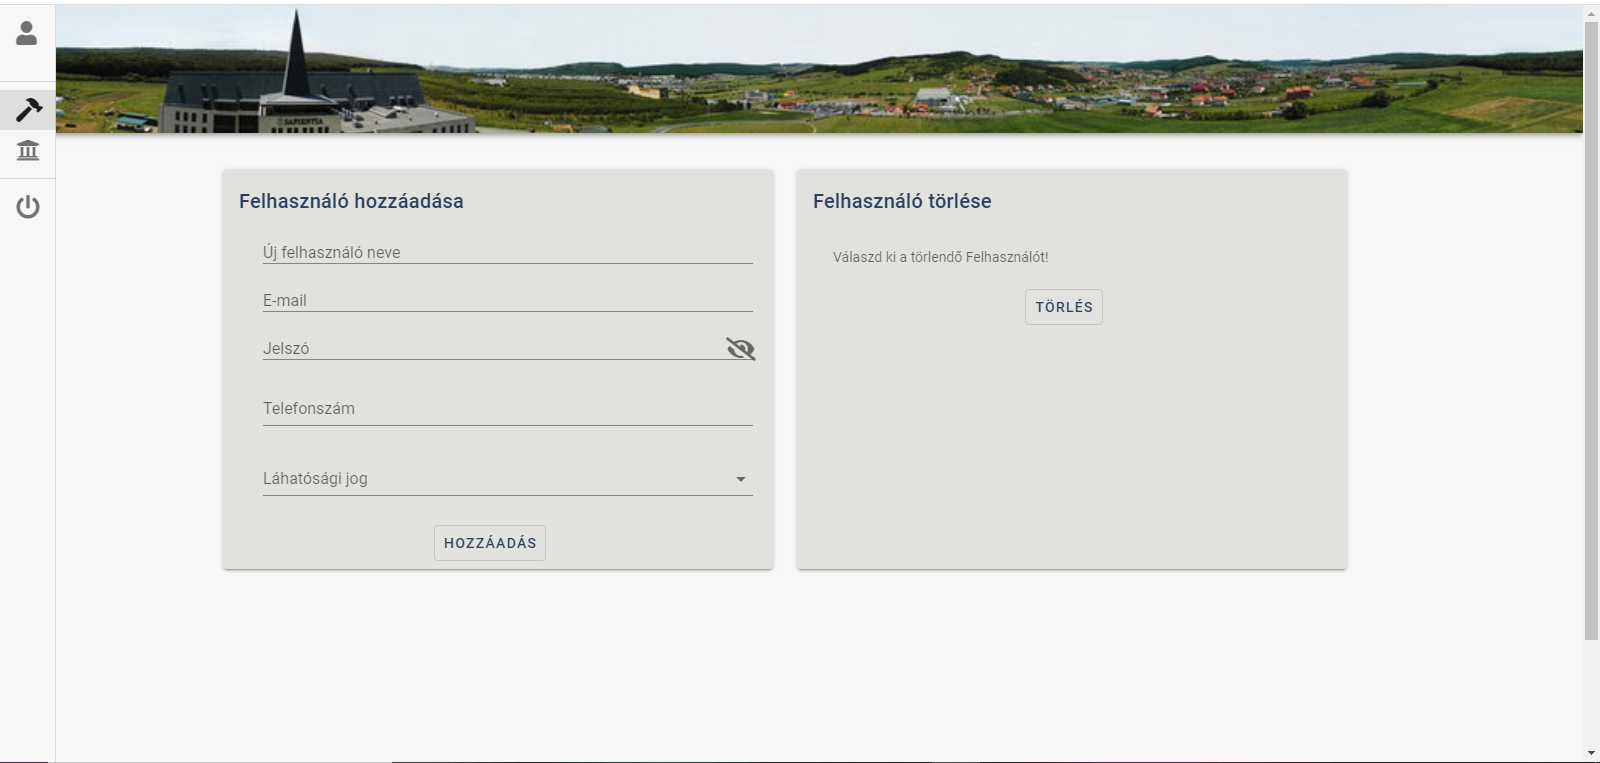
\includegraphics[scale=0.4]{figures/images/admin.png}
	\caption{A user felhasználók által használt különleges funkciók}
	\label{fig:admin}
\end{figure}
	
A következőkben azokat az elemeket mutatnám meg amelyeket minden felhasználó képes látni. Egyelőre csak egy ilyen oldal készült el és ez sem végeleges. Ezen az oldalon látható egy 3D modell amelyet a társam készített el. Megtekinthető a \ref{fig:modell} ábrán. Ezen kívül észrevehető, hogy ha nem vagyunk bejelentkezve akkor egy kicsivel másabb menürendszer jelenik meg. Ezt megtudjuk nézni a \ref{fig:drawbarevery} ábrán. A struktúra hasonló viszont itt nem jelennek meg a felhasználók adatai ámbár megjelenik a Bejelentkezés menüpont ahol be tudnak jelentkezni a felhasználók. Ez tulajdonképpen az útválasztás(rout) folyamaton belül oldódott meg. Egy útválasztás van és azon belül két nagyobb csoportra lett felosztva, hogy ki melyik oldalt láthatja. 
	
\begin{figure}
	\centering
	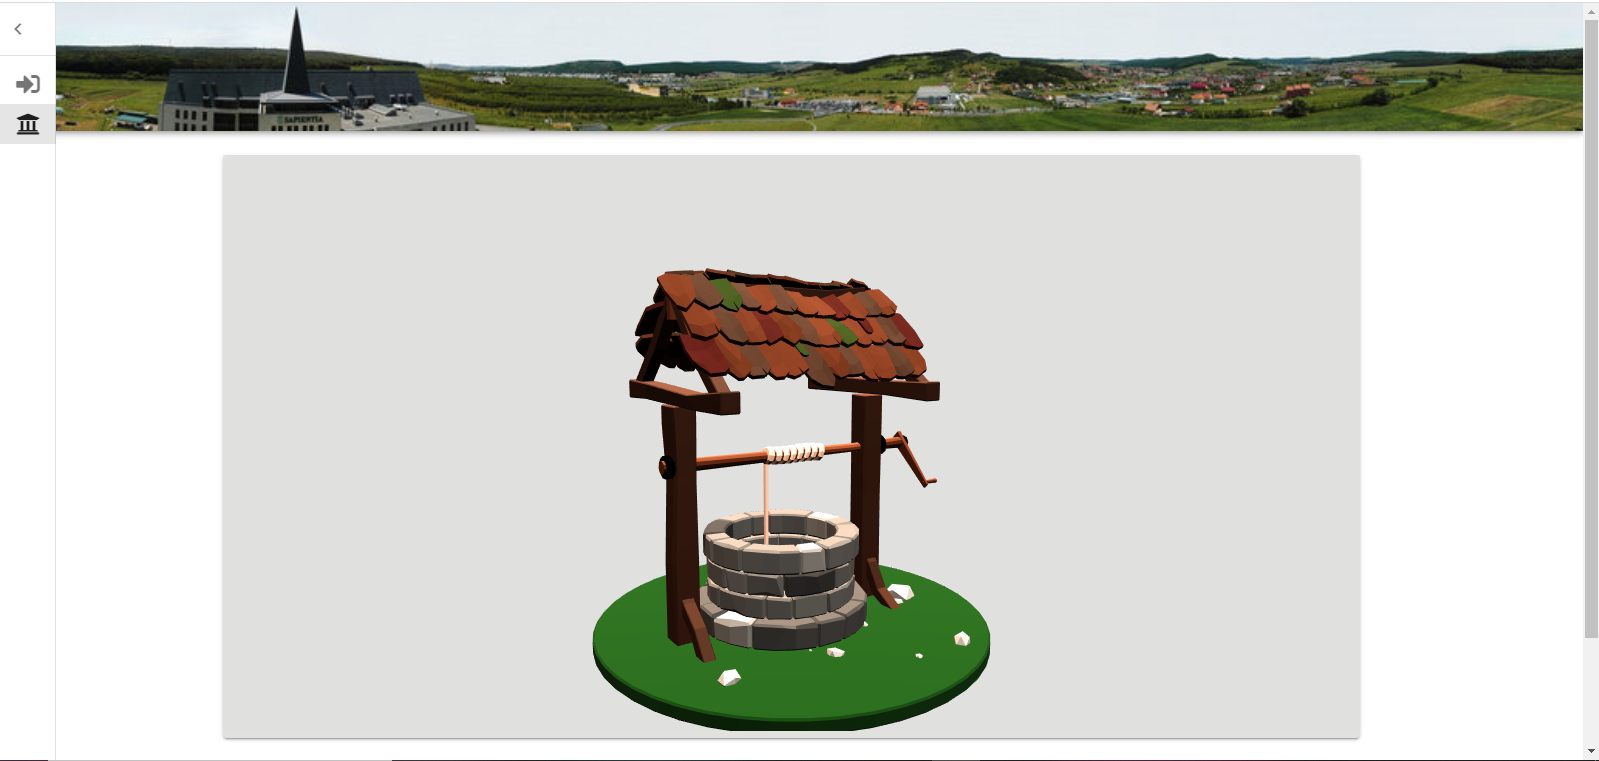
\includegraphics[scale=0.4]{figures/images/modell.png}
	\caption{A 3D modell kép visitor(látogató) és user felhasználók számára}
	\label{fig:modell}
\end{figure}

\begin{figure}
	\centering
	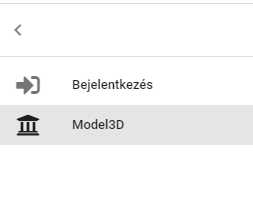
\includegraphics[scale=0.7]{figures/images/drawbarevery.png}
	\caption{Visitor(látogató) felhasználó által látható menürendszer}
	\label{fig:drawbarevery}
\end{figure}

Az alkalmazást egyelőre web felületen készítem el, mivel így a különböző eszközökön nem kell különbséget tenni. Nem kell megírni külön Android vagy IOS rendszerrel rendelkező mobiltelefonok nyelvére. A web felületre írt oldalakat megtudja nyitni az Androiddal és IOS rendszerre rendelkező ember is mivel nem kell külön alkalmazást letölteni. Ezen kívül egy weboldal elérhető számítógépen is. Fejlesztési lehetőségnek persze ott tartom azt is, hogy majd ne csak web applikáció legyen hanem Android meg IOS is. Mindkettőt hasznosnak tartom mivel világunkban a telefonok használata nagyon népszerű.